% !TeX root = ../main.tex
% Add the above to each chapter to make compiling the PDF easier in some editors.

\chapter{Hyperparameter Optimization with Sparse Grids}\label{chapter:main_part}

\section{Methodology}

\subsection{Adaptive Grid Search with Sparse Grids}

\begin{itemize}
	\item Evaluating neural networks as function with input of the hyperparameters
	\item General goals
\end{itemize}

\subsection{Implementation}

\begin{itemize}
	\item Dataset class
	\item Optimization class
		\subitem Implementation of sparse grid search with SG++
		\subitem Implementation of grid and random search
		\subitem Implementation of bayesian optimization
\end{itemize}


\section{Sparse Grid Optimization of functions}

Before optimizing the configurations of machine learning models, simple functions are used. This has the advantage that the optimal point is already known in advance and a function call is much faster than evaluating a neural network. Therefore, three different test functions are given with the following properties \cite{valentin2016hierarchical}:

\begin{table}[htbp!]
		\centering
	\begin{tabular}{|c c c c|} 
		\hline
		Function & Domain & $x_{opt}$ & $ f(x_{opt}) $\\
		\hline
		Eggholder & $[-512, 512]^2 $ & $(512, 404.2319)$ & $ -959.6407 $ \\
		Rosenbrock & $[-5, 10]^2 $ & $(1,1)$ & $ 0 $ \\
		Rastrigin & $[-2, 8]^d $ & $\vec{0}$ & $ 0 $ \\
		\hline
	\end{tabular}
	\caption{ Three test functions and their properties.}
	\label{tab:test_functions}
\end{table}

The Eggholder function is defined with \cite{whitley1996evaluating} 
\begin{equation}
	f(x_0, x_1) = -x_0 * \text{sin}(\sqrt{ | x_0 - (x_1 + 47) | }) - (x_1 + 47) \text{sin}(\sqrt{ | x_1 +47 + \frac{x_0}{2} | }).
\end{equation}

The second function (Rosenbrock) \cite{yang2010engineering} is calculated with 
\begin{equation}
	f(x_0, x_1) = (1-x_0)^2 + 100 (x_1 - x_0^2)^2.
\end{equation} 
and the third one (Rastrigin) \cite{yang2010engineering} is defined with
\begin{equation}
	f(\vec{x}) = 10 d + \sum_{ i = 1 }^{d} (x_i^2 - 10 \text{cos}(2 \pi x_i))
\end{equation} 
where $ d $ is the dimensionality of the input vector $ \vec{x} $. Figure \ref{fig:test_functions_plot} shows the functions in two dimensions.


\begin{figure}[htbp!]
	\begin{subfigure}{0.3\textwidth}
		\centering
		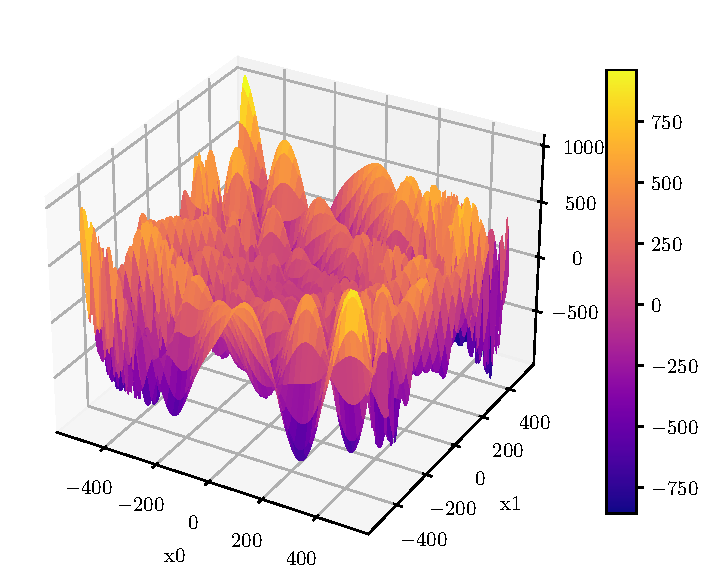
\includegraphics[width=\textwidth]{Eggholder_normal}
		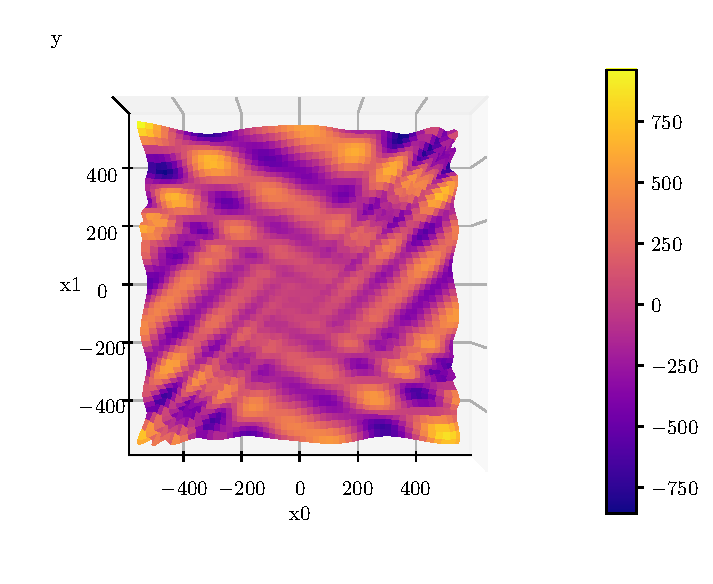
\includegraphics[width=\textwidth]{Eggholder_above}
		\caption{Eggholder.}
		\label{fig:Eggholder}
	\end{subfigure}
	\begin{subfigure}{0.3\textwidth}
		\centering
		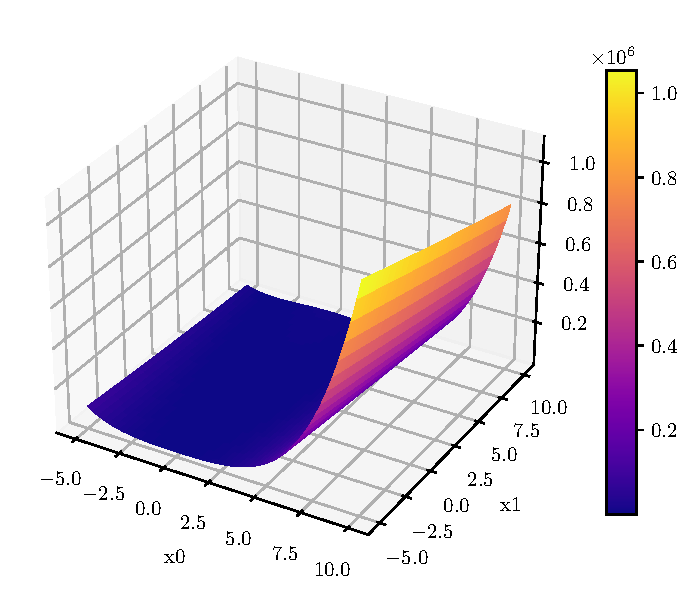
\includegraphics[width=\textwidth]{Rosenbrock_normal}
		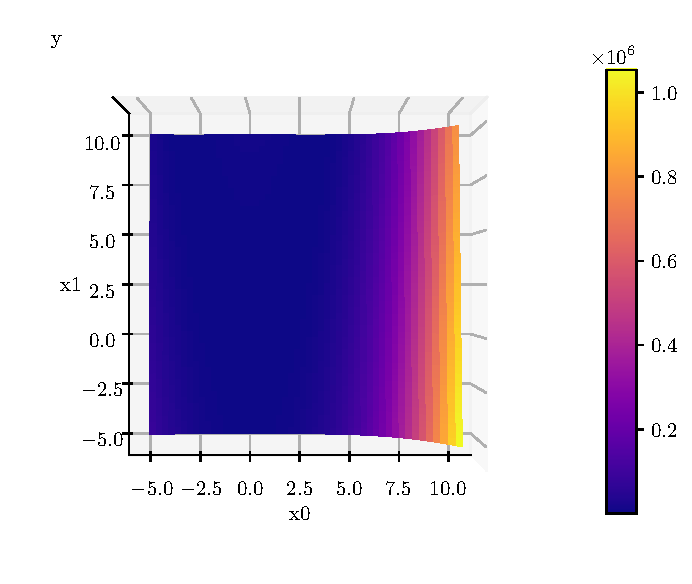
\includegraphics[width=\textwidth]{Rosenbrock_above}
		\caption{$ log_{10}(f) $ of Rosenbrock.}
		\label{fig:Rosenbrock}
	\end{subfigure}
	\begin{subfigure}{0.3\textwidth}
		\centering
		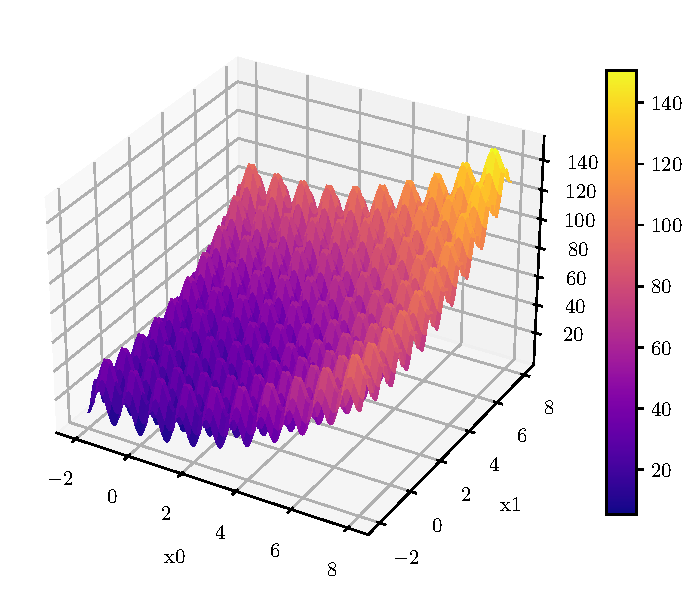
\includegraphics[width=\textwidth]{Rastrigin_normal}
		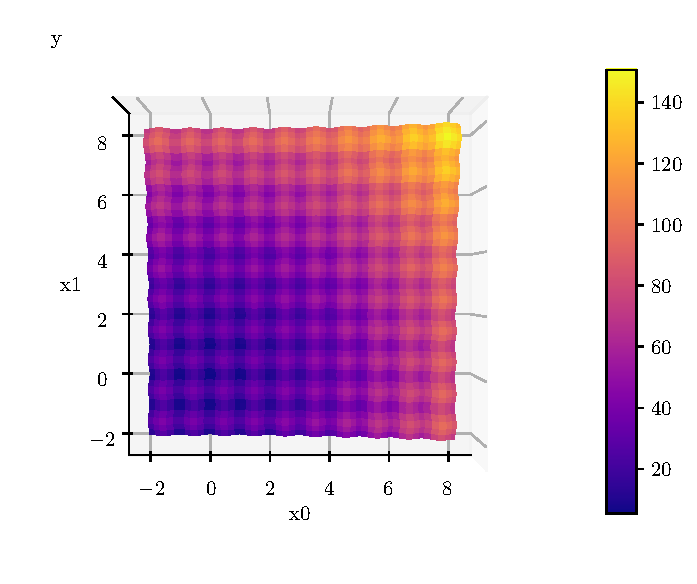
\includegraphics[width=\textwidth]{Rastrigin_above}
		\caption{Rastrigin.}
		\label{fig:Rastrigin}
	\end{subfigure}
	
	\caption{Test functions used for evaluating the sparse grid optimization. Each one is plotted with 200 samples in each dimension. Note that the function values of the Rosenbrock function are transformed with $ log_{10}(f(x)) $ for better visualization.}
	\label{fig:test_functions_plot}
\end{figure}

The Eggholder function (see Figure \ref{fig:Eggholder}) is oscillatory and the optimal point $ x_{opt} $ lays at the border of the domain. Additionally, it is multi modal. The second one (see Figure \ref{fig:Rosenbrock}) is plotted with the function values additionally transformed with $ log_{10}(x) $ for better visualization. The last one is also multi modal (see Figure \ref{fig:Rastrigin}). 

As a first step, the sparse grid generation which is done with the Ritter Novak refinement criterion \cite{b_splines} is evaluated. In each iteration, the grid point $ x_{l,i} $ that minimizes the product 
\begin{equation}
	(r_{l,i} +1)^{1 - \gamma} \cdot (||l||_1 + d_{l,i} + 1)^{\gamma}
\end{equation}
is refined. In this case, $ r_{l,i} = |\{ (l', i') \in K | f(x_{l',i'}) \le f(x_{l,i}) \}| \in \{1, ... , |K|\} $ is the rank of the grid point with $ K $ being the current set of level-index pairs of the grid. This rank denotes the place of the function value in the ascending order of all values of the current grid. On the other hand, the degree of the point $ d_{l,i} \in \mathbb{N}_0 $ is the number of previous refinements at this point. One important choice has to be made for the adaptivity parameter $ \gamma $. This value has to be between 0 and 1 and the smaller this value is, the more adaptive is the sparse grid. With this value, a trade-off between exploration and exploitation can be balanced. The optimal value generally depends on the function that has to be optimized. \newline

\subsection{Sparse Grid Generation with different Adaptivities}

In the following, the behavior of the sparse grid generation is analyzed with the help of the three test functions. In each case, 3 different values for the adaptivity parameter $ \gamma \in \{0.0, 0.5, 1.0\} $ are used and the resulting sparse grid with the triangulated function values is plotted. The first test case is the Eggholder function and the result is depicted in Figure \ref{fig:Eggholder_grid}.

\begin{figure}[htbp!]
	\begin{subfigure}{0.3\textwidth}
		\centering
		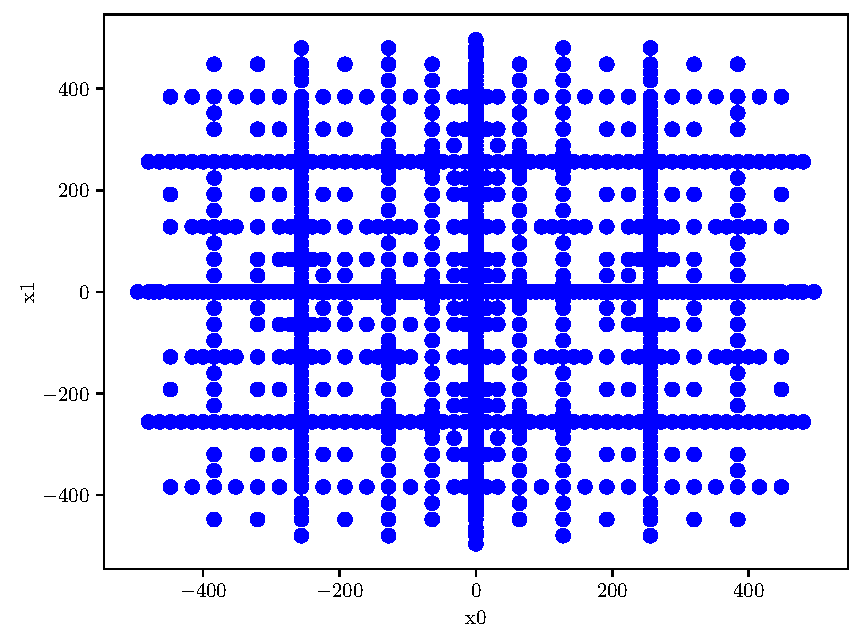
\includegraphics[width=\textwidth]{figures/Results/Sparse_grid_generation_results/Eggholder/tex_files/Eggholder_1}
		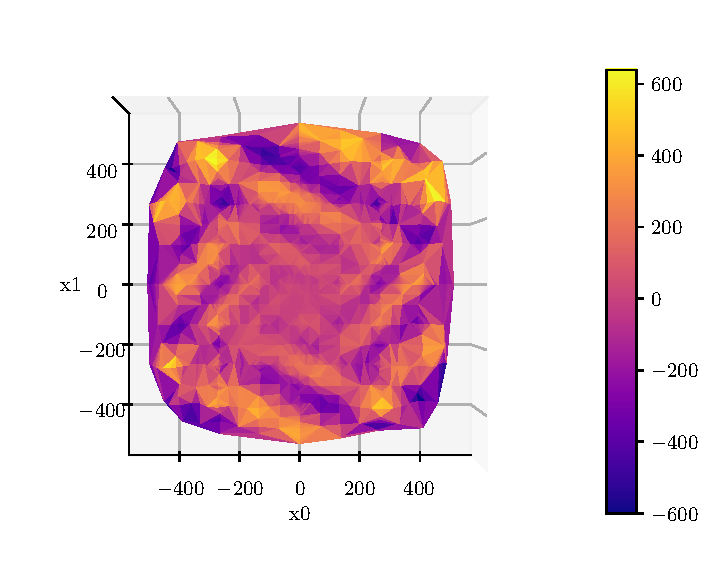
\includegraphics[width=\textwidth]{figures/Results/Sparse_grid_generation_results/Eggholder/tex_files/Eggholder_above_1}
		\caption{$ \gamma = 1.0 $}
		\label{fig:Egg_gamma_1}
	\end{subfigure}
	\begin{subfigure}{0.3\textwidth}
		\centering
		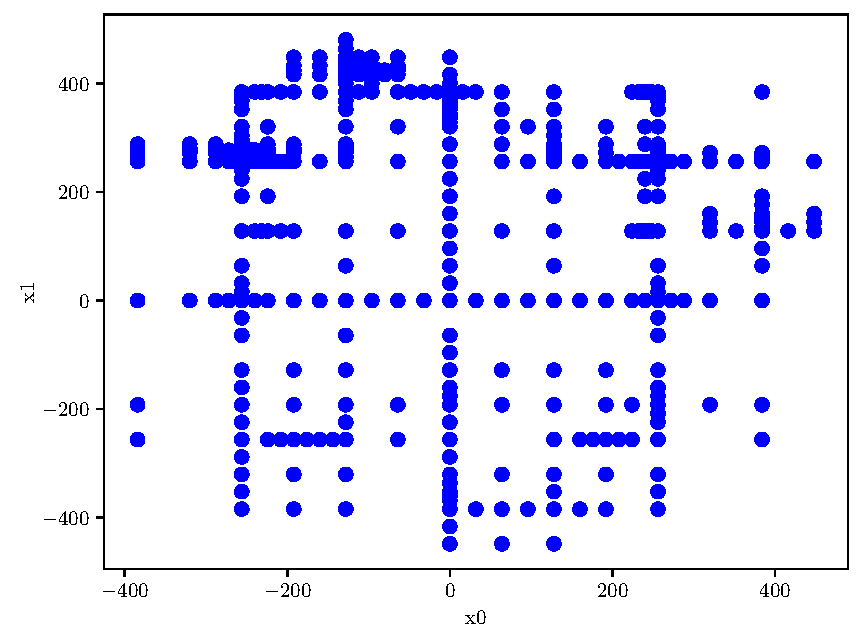
\includegraphics[width=\textwidth]{figures/Results/Sparse_grid_generation_results/Eggholder/tex_files/Eggholder_0_5}
		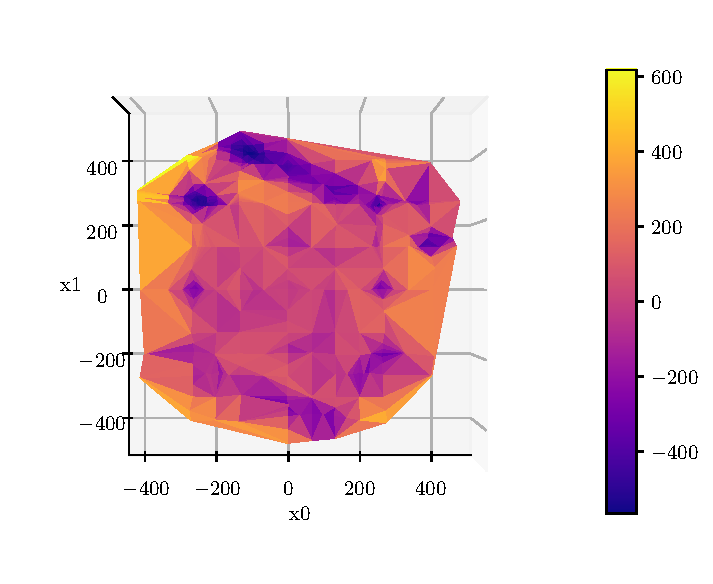
\includegraphics[width=\textwidth]{figures/Results/Sparse_grid_generation_results/Eggholder/tex_files/Eggholder_above_0_5}
		\caption{$ \gamma = 0.5 $}
		\label{fig:Egg_gamma_0_5}
	\end{subfigure}
	\begin{subfigure}{0.3\textwidth}
		\centering
		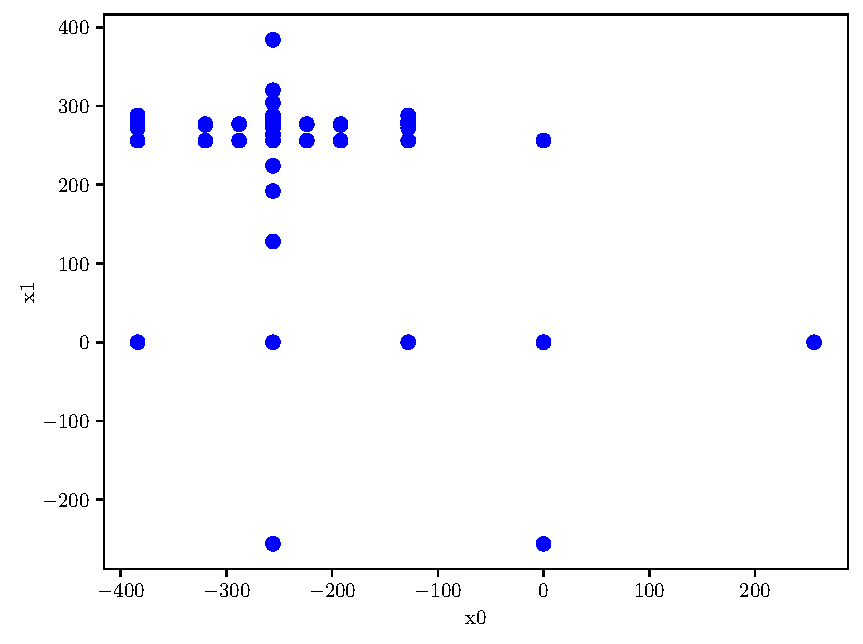
\includegraphics[width=\textwidth]{figures/Results/Sparse_grid_generation_results/Eggholder/tex_files/Eggholder_0}
		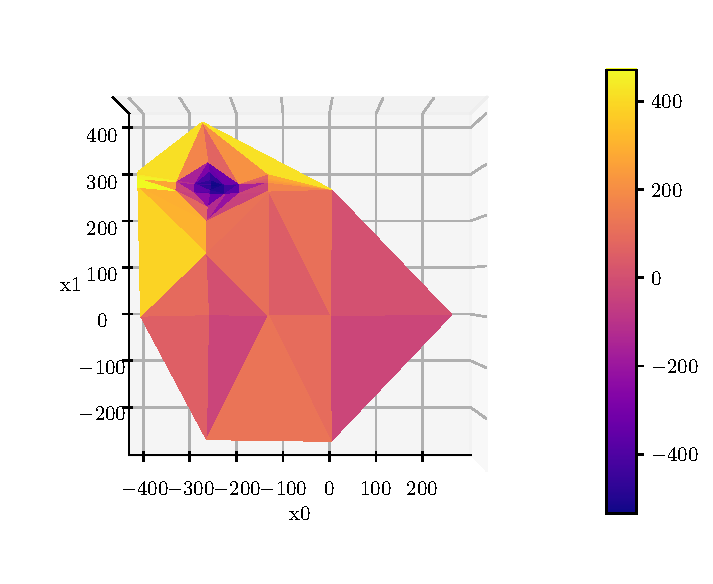
\includegraphics[width=\textwidth]{figures/Results/Sparse_grid_generation_results/Eggholder/tex_files/Eggholder_above_0}
		\caption{$ \gamma = 0.0 $}
		\label{fig:Egg_gamma_0}
	\end{subfigure}
	
	\caption{Sparse grid generation depending on the adaptivity parameter $ \gamma $ for the Eggholder function. In all cases, the same number of grid points is used. Here, in each of the 249 iterations, 4 new grid points are added resulting in a overall number of 997 function evaluations.}
	\label{fig:Eggholder_grid}
\end{figure}

In the first case with $ \gamma = 1.0 $, the grid is homogeneous and not adaptive at all. The grid points are distributed over the whole domain and the interpolated function looks very similar to the real plot from Figure \ref{fig:Eggholder}. 

The other extreme case is depicted in Figure \ref{fig:Egg_gamma_0}. There, the grid is maximally adaptive and really concentrated at the top left corner around $ (-260, 280) $. As it is known from Table \ref{tab:test_functions}, this is not where the optimal point is located. This behavior can be explained by the high exploitation throughout the iterations. With such a low adaptivity parameter, the grid points with low function values in the first iterations are mostly refined in the other iteration steps. 

The middle case with $ \gamma = 0.5 $ depicts a case where exploitation and exploration are more balanced. The grid points are more distributed than in the case of $ \gamma = 0.0 $ but there are also some regions where they are more refined, e.g. in the top left corner of the domain.

Note that in all three cases, the exact same number of grid points are evaluated. In this case it is very hard for the sparse grid to find the real optimum because it is located at the border of the domain and it does not use grid points at the border. Also, the oscillatory nature of the function makes it hard to not concentrate on a local optimum which can happen in case of too high adaptivity. \newline

The next function used is the Rosenbrock function (see Figure \ref{fig:Rosenbrock}). Again, three different values for the adaptivity parameter are used. The results are depicted in Figure \ref{fig:Rosenbrock_grid}.

\begin{figure}[htbp!]
	\begin{subfigure}{0.3\textwidth}
		\centering
		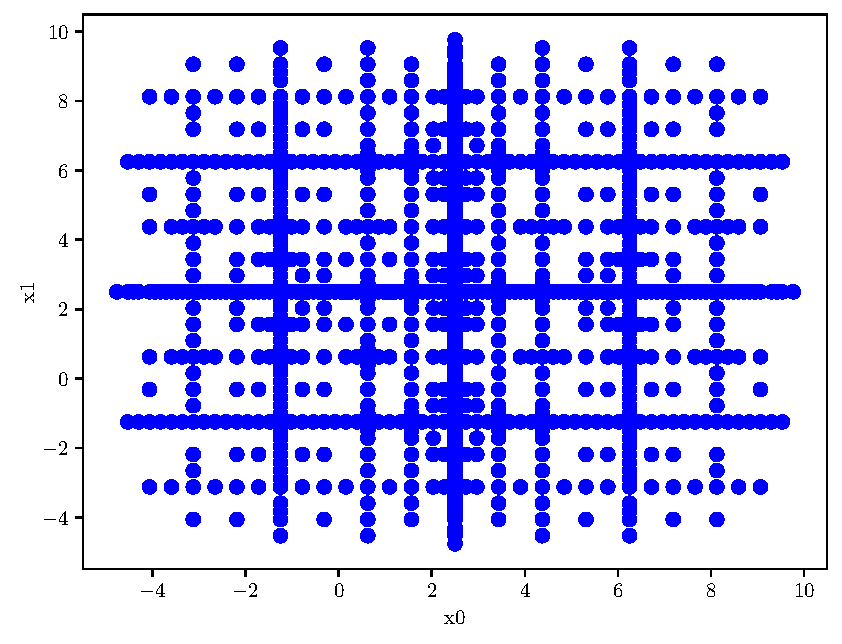
\includegraphics[width=\textwidth]{figures/Results/Sparse_grid_generation_results/Rosenbrock/tex_files/Rosenbrock_1}
		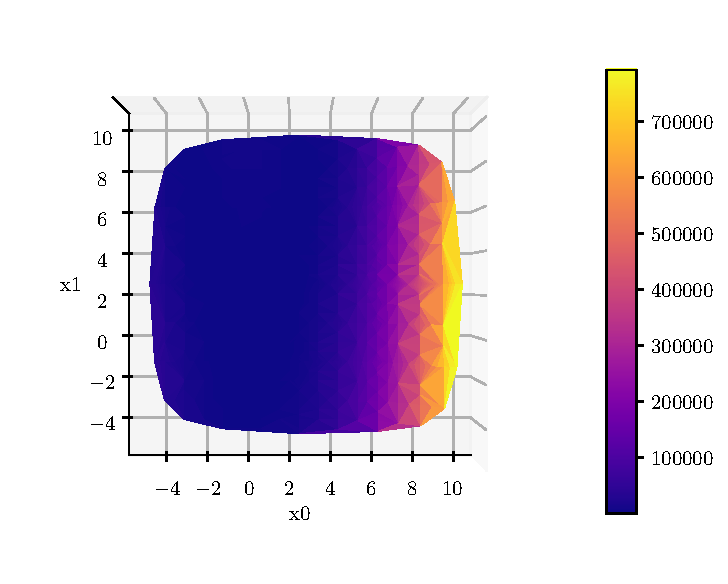
\includegraphics[width=\textwidth]{figures/Results/Sparse_grid_generation_results/Rosenbrock/tex_files/Rosenbrock_above_1}
		\caption{$ \gamma = 1.0 $}
		\label{fig:Ros_gamma_1}
	\end{subfigure}
	\begin{subfigure}{0.3\textwidth}
		\centering
		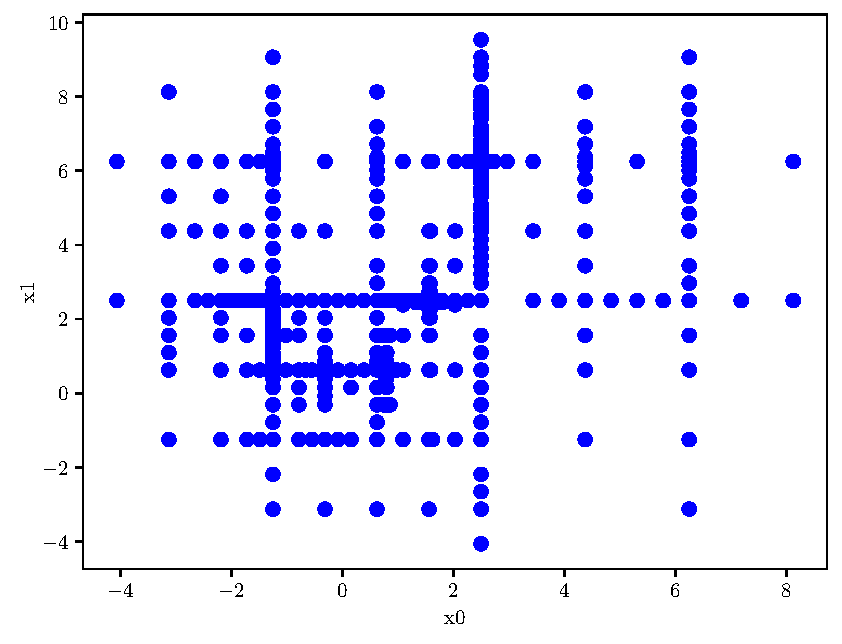
\includegraphics[width=\textwidth]{figures/Results/Sparse_grid_generation_results/Rosenbrock/tex_files/Rosenbrock_0_5}
		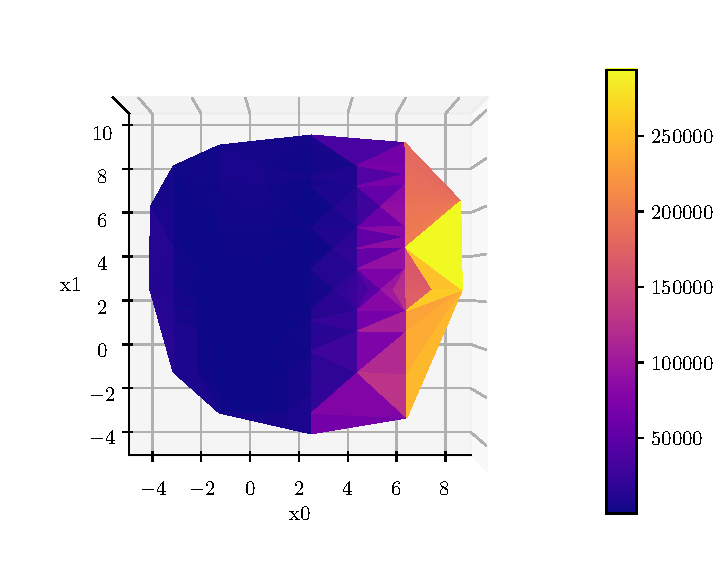
\includegraphics[width=\textwidth]{figures/Results/Sparse_grid_generation_results/Rosenbrock/tex_files/Rosenbrock_above_0_5}
		\caption{$ \gamma = 0.5 $}
		\label{fig:Ros_gamma_0_5}
	\end{subfigure}
	\begin{subfigure}{0.3\textwidth}
		\centering
		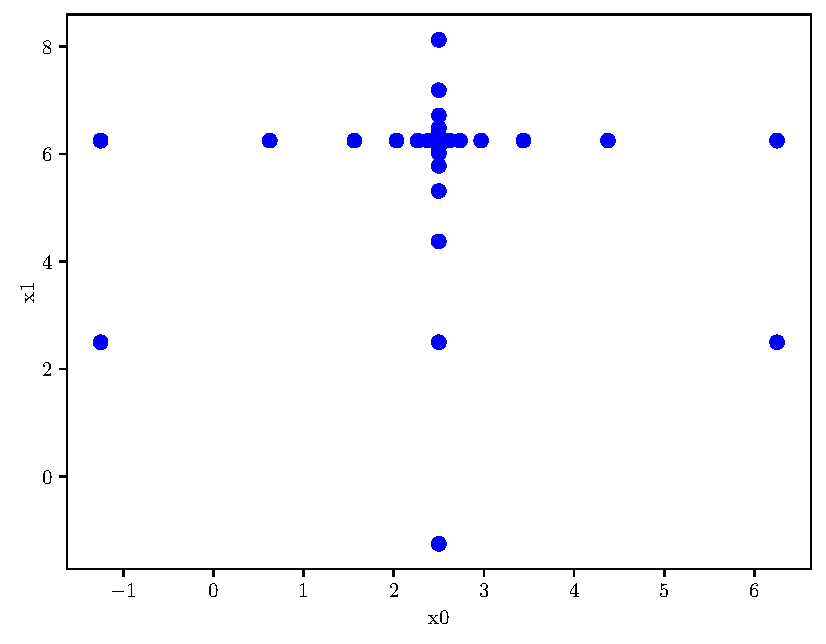
\includegraphics[width=\textwidth]{figures/Results/Sparse_grid_generation_results/Rosenbrock/tex_files/Rosenbrock_0}
		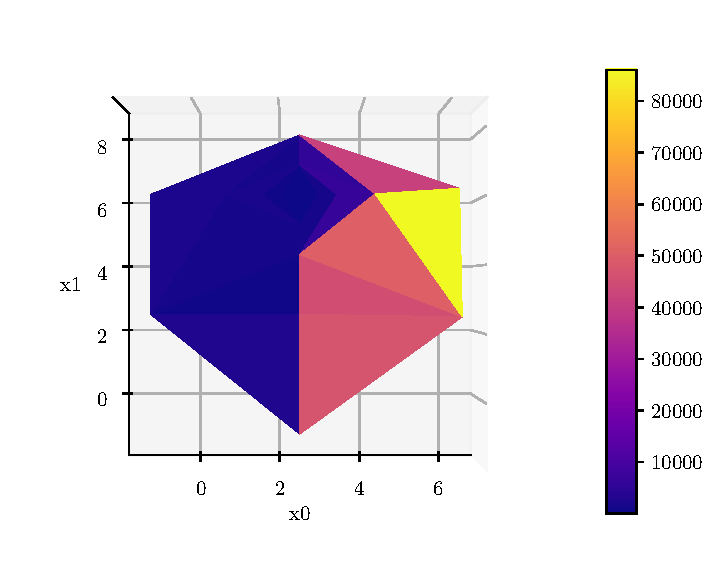
\includegraphics[width=\textwidth]{figures/Results/Sparse_grid_generation_results/Rosenbrock/tex_files/Rosenbrock_above_0}
		\caption{$ \gamma = 0.0 $}
		\label{fig:Ros_gamma_0}
	\end{subfigure}
	
	\caption{Sparse grid generation depending on the adaptivity parameter $ \gamma $ for the Rosenbrock function. In all cases, the same number of grid points is used. Here, in each of the 249 iterations, 4 new grid points are added resulting in a overall number of 997 function evaluations.}
	\label{fig:Rosenbrock_grid}
\end{figure}


The first fact that can be observed is that the sparse grid in the first case (Figure \ref{fig:Ros_gamma_1}) is exactly the same as the one for the Eggholder function (Figure \ref{fig:Egg_gamma_1}). This is due to the fact that this value of $ \gamma $ leads to a homogeneous sparse grid which is not dependent on the function used but rather the number of iterations for the grid generation. In this case, the interpolated function looks similar to the real function (Figure \ref{fig:Rosenbrock}). 

Now with decreasing value of $ \gamma $, the grid gets more and more inhomogeneous, while concentrating to refine smaller function values. The extreme case can be seen in Figure \ref{fig:Ros_gamma_0}, where the most grid points are next to the point $ (2.5, 6.25) $. After refining the first point in the middle, the one on top of it is getting refined all the time for the case $ \gamma = 0.0 $. Again, the sparse grid with $ \gamma = 0.5 $ is more balanced with more grid points on the left where the real optimum is located. \newline 


The last function used is the Rastrigin function (see Figure \ref{fig:Rastrigin} for the plot of the function and \ref{fig:Rastrigin_grid} for the resulting sparse grids). 

\begin{figure}[htbp!]
	\begin{subfigure}{0.3\textwidth}
		\centering
		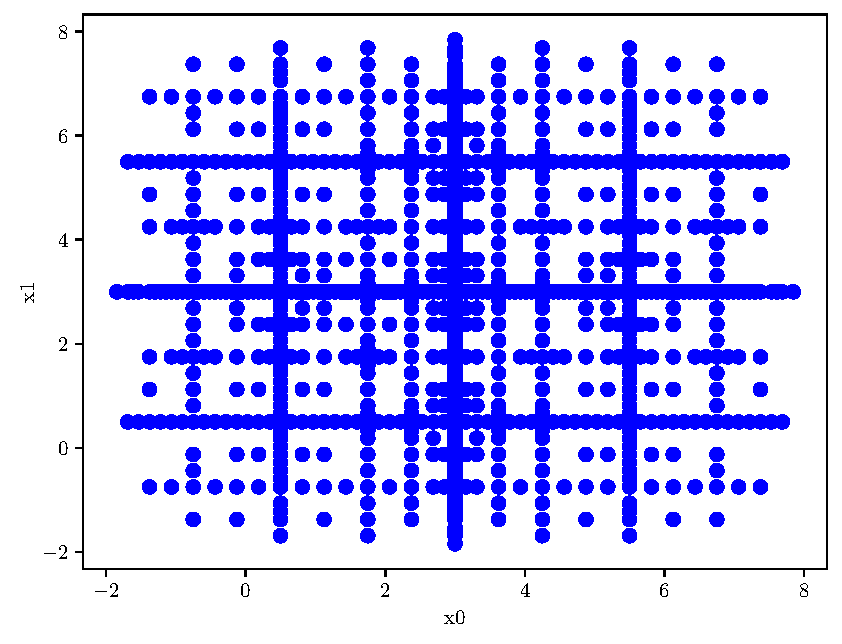
\includegraphics[width=\textwidth]{figures/Results/Sparse_grid_generation_results/Rastrigin/tex_files/Rastrigin_1}
		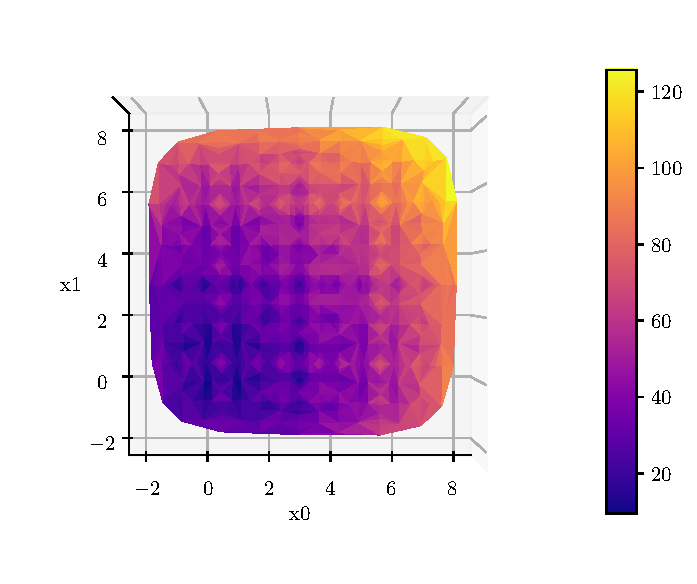
\includegraphics[width=\textwidth]{figures/Results/Sparse_grid_generation_results/Rastrigin/tex_files/Rastrigin_above_1}
		\caption{$ \gamma = 1.0 $}
		\label{fig:Ras_gamma_1}
	\end{subfigure}
	\begin{subfigure}{0.3\textwidth}
		\centering
		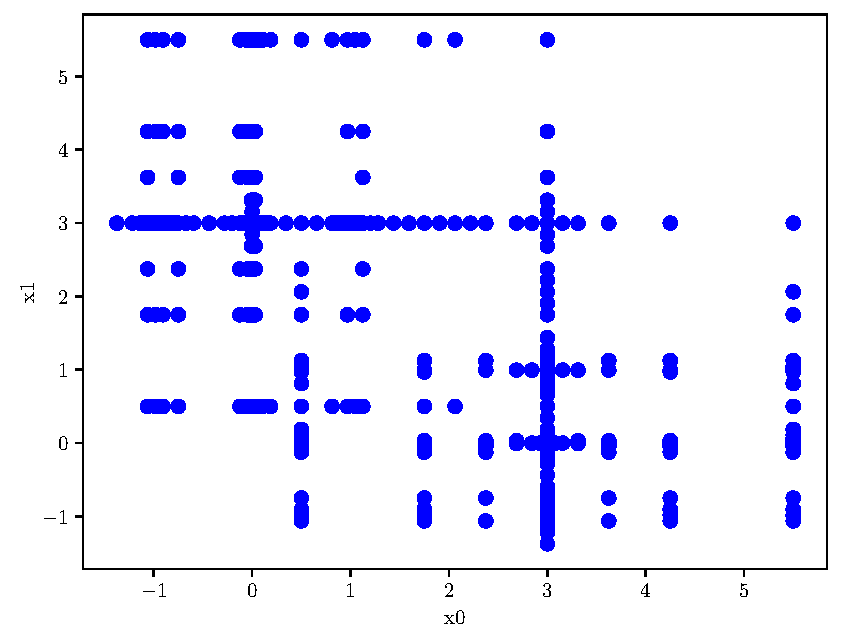
\includegraphics[width=\textwidth]{figures/Results/Sparse_grid_generation_results/Rastrigin/tex_files/Rastrigin_0_5}
		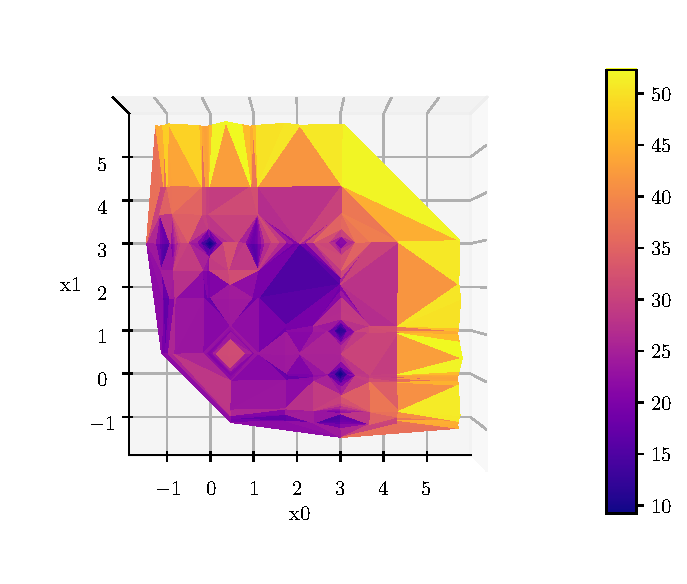
\includegraphics[width=\textwidth]{figures/Results/Sparse_grid_generation_results/Rastrigin/tex_files/Rastrigin_above_0_5}
		\caption{$ \gamma = 0.5 $}
		\label{fig:Ras_gamma_0_5}
	\end{subfigure}
	\begin{subfigure}{0.3\textwidth}
		\centering
		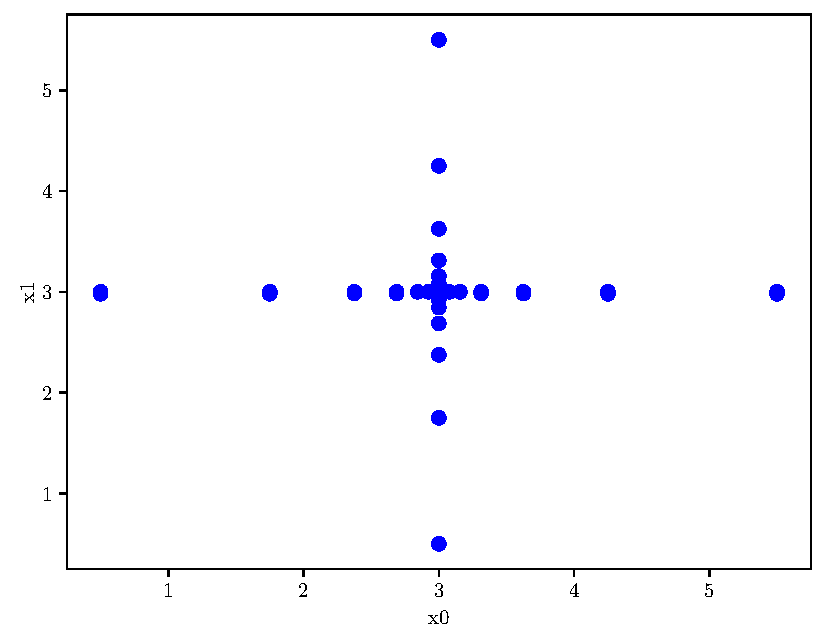
\includegraphics[width=\textwidth]{figures/Results/Sparse_grid_generation_results/Rastrigin/tex_files/Rastrigin_0}
		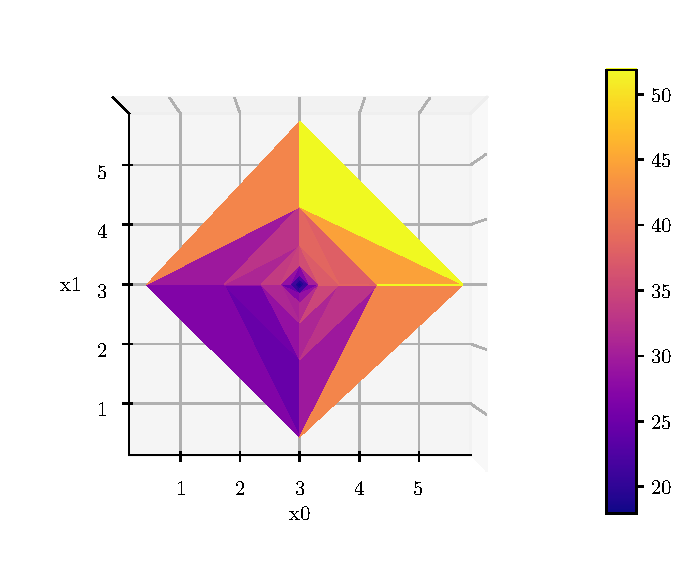
\includegraphics[width=\textwidth]{figures/Results/Sparse_grid_generation_results/Rastrigin/tex_files/Rastrigin_above_0}
		\caption{$ \gamma = 0.0 $}
		\label{fig:Ras_gamma_0}
	\end{subfigure}
	
	\caption{Sparse grid generation depending on the adaptivity parameter $ \gamma $ for the Rastrigin function. In all cases, the same number of grid points is used. Here, in each of the 249 iterations, 4 new grid points are added resulting in a overall number of 997 function evaluations.}
	\label{fig:Rastrigin_grid}
\end{figure}

As in the previous two cases, the sparse grid is exactly the same for $ \gamma = 1.0 $. We can also see the same behavior for a decreasing adaptivity parameter. For $ \gamma = 0.0 $, only the grid point in the center is refined in all steps. In the middle case, the grid looks more balanced with tendency to the bottom left corner.  \newline 


In conclusion, these experiments show that the value for the adaptivity parameter strongly influences the grid generation and the resulting optimal value found by the algorithm. In general, this trade-off between exploitation with trying to find a solution fast and exploration with reconstructing the function in the whole domain can be balanced with this adaptivity parameter. \newline

In the following, the goal is to further analyze this adaptivity parameter. For each of the three test functions, experiments with $ \gamma \in \{0.0, 0.25, 0.5, 0.75, 1.0\} $ are made. The error of the optimum found by the grid is calculated depending on the number of grid points used. It is evaluated with 
\begin{equation}
 Error = f(x_{opt}^*) - f(x_{opt}) 
\end{equation}
where $ x_{opt}^* $ is the optimal point found by the sparse grid and $ x_{opt} $ is the real optimum. Figure \ref{fig:test_functions_plot} shows the resulting Errors depending on the number of grid points used. The top left plot is for the Eggholder function, the one on the top right belongs to the Rosenbrock function and the bottom one corresponds to the Rastrigin function. \newline

\begin{figure}[htbp!]
	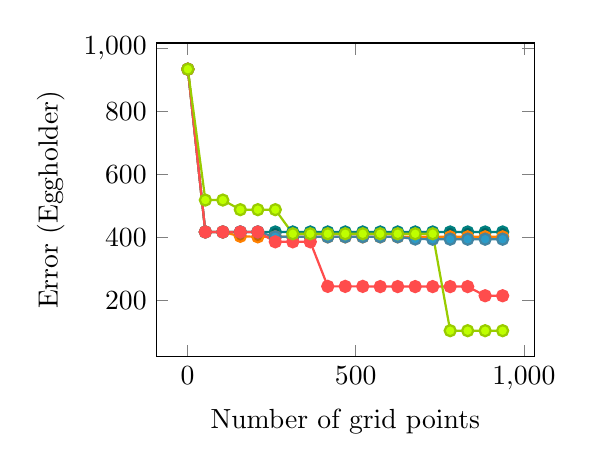
\begin{tikzpicture}
		\begin{axis}[
			xlabel = Number of grid points,
			ylabel = Error (Eggholder),
			scale=0.7,
			cycle list name=exotic,
			]
			
			\addplot+[mark=*, style=thick] coordinates {(1,934.1803628147137)(53,416.6753127436343)(105,416.67517650515606)(157,416.67517650515606)(209,416.6751765051557)(261,416.6751765051555)(313,416.67517650515515)(365,416.67517650515583)(417,416.67517650515606)(469,416.67517650515515)(521,416.67517650515595)(573,416.6751765051555)(625,416.6751765051557)(677,416.6751765051554)(729,416.6751765051555)(781,416.67517650515595)(833,416.6751765051555)(885,416.6751765051557)(937,416.6751765051557)};
			
			\addplot+[mark=*, style=thick]  coordinates 
			{(1,934.1803628147137)(53,416.6753127436343)(105,416.67517650515606)(157,402.86392358909313)(209,401.165066632121)(261,401.16506654901593)(313,401.16506654901764)(365,401.1650665490138)(417,401.1650665490125)(469,401.1650665490105)(521,401.16506654901195)(573,401.1650665490175)(625,401.16506654902184)(677,401.16506654901843)(729,401.16506654901593)(781,401.1650665490224)(833,401.16506654902105)(885,401.1650665490139)(937,401.1650665490138)};
			
			\addplot+[mark=*, style=thick]   coordinates 
			{(1,934.1803628147137)(53,416.6753127436343)(105,416.67517650515595)(157,416.67517650515595)(209,416.6751765051556)(261,401.16506923718293)(313,401.1650665490133)(365,401.1650665490122)(417,401.16506654901445)(469,401.1650665490125)(521,401.16506654901264)(573,401.16506654901264)(625,401.1650665490216)(677,394.1301115312152)(729,393.6496427441624)(781,393.6444455890784)(833,393.6437130885647)(885,393.6437130885688)(937,393.6437130885528)};
			
			\addplot+[mark=*, style=thick]  coordinates
				{(1,934.1803628147137)(53,416.680649645461)(105,416.67519174547897)(157,416.6751765051557)(209,416.6751765051554)(261,385.37674780492864)(313,385.35652906792404)(365,385.3565290679238)(417,243.68003942485666)(469,243.67992321536838)(521,243.67992321536633)(573,243.01108728703605)(625,242.99463717547087)(677,242.99463717547076)(729,242.99463717547087)(781,242.99463717546962)(833,242.99463717546973)(885,213.83490792055488)(937,213.834907133721)};
			
			\addplot+[mark=*, style=thick]  coordinates 
			{(1,934.1803628147137)(53,518.1399491004825)(105,518.1399491004823)(157,487.54622876272015)(209,487.54622876272003)(261,487.54622876272)(313,410.9897867087419)(365,410.9897867087424)(417,410.9897867087427)(469,410.9897867087419)(521,410.9897867087424)(573,410.98978670874214)(625,410.9897867087425)(677,410.9897867087424)(729,410.9897867087428)(781,102.75674102278083)(833,102.7567410227864)(885,102.75674102278651)(937,102.75674102279345)};
			
		\end{axis}
	\end{tikzpicture}
	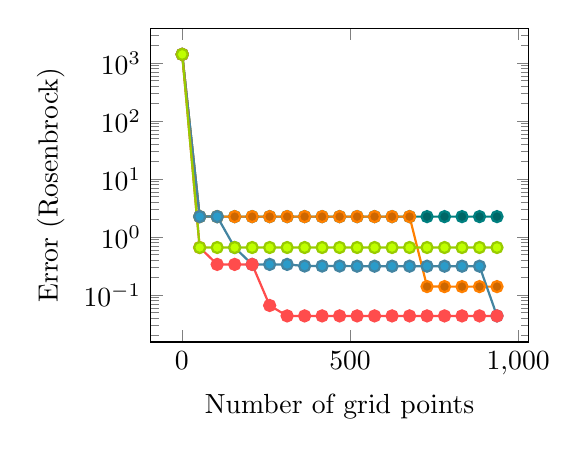
\begin{tikzpicture}
		\begin{axis}[
			xlabel = Number of grid points,
			ylabel = Error (Rosenbrock),
			scale = 0.7,
			ymode=log,
			cycle list name=exotic,
			]
			
			\addplot+[mark=*, style=thick] coordinates {(1,1408.5)(53,2.25)(105,2.2491001457701714)(157,2.2491001457701714)(209,2.2491001457722626)(261,2.2491001457672675)(313,2.249100145771435)(365,2.249100145769731)(417,2.2491001457715205)(469,2.249100145772637)(521,2.2491001457718287)(573,2.249100145770883)(625,2.2491001457697997)(677,2.24910014577051)(729,2.2491001457706186)(781,2.249100145769841)(833,2.2491001457692894)(885,2.249100145769003)(937,2.2491001457706337)};
			
			\addplot+[mark=*, style=thick]  coordinates 
			{(1,1408.5)(53,2.25)(105,2.2491001457701714)(157,2.2491001457701714)(209,2.2491001457721036)(261,2.2491001457695767)(313,2.249100145770952)(365,2.2491001457690514)(417,2.2491001457697983)(469,2.2491001457687094)(521,2.2491001457707274)(573,2.249100145770689)(625,2.2491001457705138)(677,2.249100145770712)(729,0.13999960097248135)(781,0.13973409018662308)(833,0.1397340901880652)(885,0.1397340901910032)(937,0.13973409019308297)};
			
			\addplot+[mark=*, style=thick]   coordinates 
			{(1,1408.5)(53,2.25)(105,2.2491001457701714)(157,0.65972900390625)(209,0.33738539328720274)(261,0.337384855010467)(313,0.3373848550084554)(365,0.3164062500005624)(417,0.3160824744022442)(469,0.316082474402264)(521,0.3143689789723247)(573,0.31436571579881106)(625,0.3143657157996295)(677,0.3143657157842261)(729,0.3143657158217291)(781,0.31436571578093114)(833,0.3143657158159762)(885,0.31436571582376066)(937,0.04369918730841191)};
			
			\addplot+[mark=*, style=thick]  coordinates
			{(1,1408.5)(53,0.65972900390625)(105,0.33738539328578554)(157,0.3373848550099865)(209,0.33738485500900234)(261,0.06609634402749087)(313,0.04368661484965771)(365,0.043686614913836186)(417,0.043686614861208506)(469,0.04368661485251346)(521,0.04368661485326686)(573,0.04368661485538938)(625,0.04368661485308678)(677,0.043686614838481574)(729,0.04368661486120118)(781,0.04368661488831904)(833,0.043686614839174354)(885,0.04368661486845582)(937,0.04368661486256009)};
			
			\addplot+[mark=*, style=thick]  coordinates 
			{(1,1408.5)(53,0.65972900390625)(105,0.65972900390625)(157,0.65972900390625)(209,0.6597290039064774)(261,0.6597290039068184)(313,0.65972900390625)(365,0.65972900390625)(417,0.65972900390625)(469,0.6597290039065911)(521,0.6597290039067047)(573,0.6597290039064774)(625,0.6597290039064774)(677,0.6597290039067047)(729,0.6597290039067047)(781,0.6597290039064774)(833,0.65972900390625)(885,0.6597290039065911)(937,0.6597290039065911)};
			
		\end{axis}
	\end{tikzpicture}
	\centering
	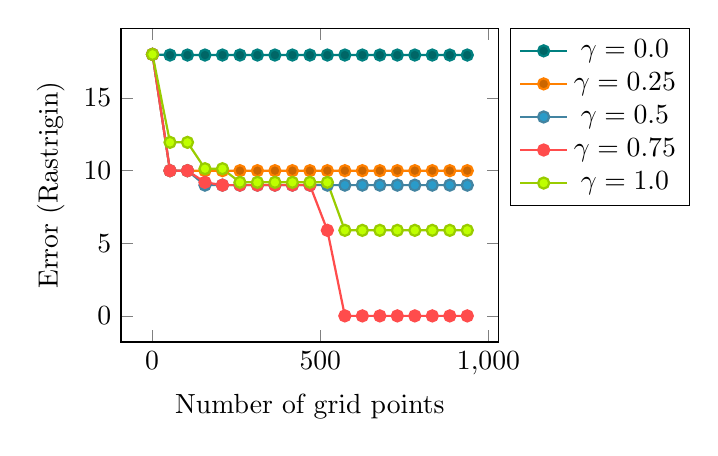
\begin{tikzpicture}
		\begin{axis}[
			xlabel = Number of grid points,
			ylabel = Error (Rastrigin),
			scale = 0.7,
			cycle list name=exotic,
			legend pos=outer north east,
			]
			
			\addplot+[mark=*, style=thick] coordinates{(1,18.0)(53,17.954603830243304)(105,17.954601241487484)(157,17.954601241487484)(209,17.95460124148829)(261,17.954601241487573)(313,17.95460124148752)(365,17.954601241487435)(417,17.95460124148751)(469,17.954601241487524)(521,17.954601241487467)(573,17.954601241487463)(625,17.954601241487506)(677,17.954601241487463)(729,17.95460124148793)(781,17.954601241488138)(833,17.954601241487886)(885,17.954601241487513)(937,17.954601241488046)};
			
			\addplot+[mark=*, style=thick]  coordinates 
			{(1,18.0)(53,9.995024358227056)(105,9.994959057644616)(157,9.994959057644616)(209,9.994959057646103)(261,9.99495905764463)(313,9.994959057644524)(365,9.99495905764453)(417,9.99495905764462)(469,9.994959057644579)(521,9.994959057644468)(573,9.994959057644502)(625,9.994959057644628)(677,9.994959057644607)(729,9.99495905764461)(781,9.994959057644595)(833,9.99495905764462)(885,9.994959057644616)(937,9.994959057644667)};
			
			\addplot+[mark=*, style=thick]   coordinates 
			{(1,18.0)(53,9.995024358227056)(105,9.994959057644618)(157,9.000000184767032)(209,9.000000000721773)(261,9.0000000007217)(313,9.000000000721338)(365,9.000000000721721)(417,9.00000000072155)(469,9.00000000072114)(521,9.000000000721972)(573,9.000000000721784)(625,9.00000000072177)(677,9.000000000721762)(729,9.00000000072182)(781,9.000000000721915)(833,9.000000000721828)(885,9.000000000721684)(937,9.000000000721721)};
			
			\addplot+[mark=*, style=thick]  coordinates
			{(1,18.0)(53,9.995597577515051)(105,9.994959320973711)(157,9.193123758467696)(209,9.000000000721291)(261,9.000000000720725)(313,9.00000000073414)(365,9.000000000715445)(417,9.000000000715788)(469,9.00000000072136)(521,5.889114376269022)(573,0.001513592628570368)(625,1.9994962252604298e-07)(677,1.2455895805700494e-08)(729,1.2778394708011167e-08)(781,1.2291804361994243e-08)(833,1.179890717001382e-08)(885,1.251678228282502e-08)(937,1.231146666513552e-08)};
			
			\addplot+[mark=*, style=thick]  coordinates 
			{(1,18.0)(53,11.944557188134524)(105,11.944557188134521)(157,10.130623758467696)(209,10.130623758467692)(261,9.193123758467797)(313,9.193123758467703)(365,9.193123758467696)(417,9.1931237584677)(469,9.1931237584677)(521,9.193123758467692)(573,5.8891143762690925)(625,5.889114376269034)(677,5.88911437626902)(729,5.889114376269047)(781,5.889114376269048)(833,5.889114376269062)(885,5.889114376269007)(937,5.889114376269115)};
			
			\legend{$ \gamma = 0.0 $, $ \gamma = 0.25 $, $ \gamma = 0.5 $, $ \gamma = 0.75 $, $ \gamma = 1.0 $,}
			
		\end{axis}
	\end{tikzpicture}
	\caption{ Influence of the adaptivity parameter on the error (difference to the actual optimal value) of the optimum found by the sparse grid. }	
	\label{fig:Functions_results}
\end{figure}

For all three test functions, a value $ 0.75 \le \gamma \le 1.0 $ leads to the smallest error with higher number of grid points. This means that a fast exploitation is not good for finding the global optimum. For the Rastrigin function, the most adaptive sparse grid does not even lead to a smaller error with up to 1000 grid points. This is the same example as in Figure \ref{fig:Ras_gamma_0}, where only the center point is refined. Note that by now, no optimization algorithm is applied on top of the sparse grid. For further experiments, the adaptivity parameter will be set to $ \gamma = 0.85 $. \newline 

\subsection{Local and Global Optimization}

The next improvement is to add optimizers after the grid generation phase. There are two different types of algorithms. The first one is local optimization, for example based on the gradient like gradient descent. The second one is global optimization. An example therefore is to use a multi start approach by trying out multiple different starting points for the algorithm. These various initial values can be uniformly distributed in the domain. The following experiments show how the error (difference between optimum found by algorithm and actual optimal function value) behaves with higher number of grid points of the underlying sparse grid. As a local optimization algorithm, the gradient descent is used. The starting point for this algorithm is set to the point of the sparse grid where the smallest function value was found. For the global optimization, a multi start approach with 20 equally distributed starting points is used. The concrete algorithm is the nelder mead optimization as described in \ref{Optimization_algorithms}. The number of function evaluations used in this method, as well as the number of steps for gradient descent is set to 1000. One important parameter for the optimization is the degree of the B-splines used on the sparse grid. The resulting errors depending on the number of grid points for the degrees 2, 3, and 5 can be seen in Figure \ref{fig:Optimizer_results}. The Rosenbrock function is used in all cases.

\begin{figure}[htbp!]
	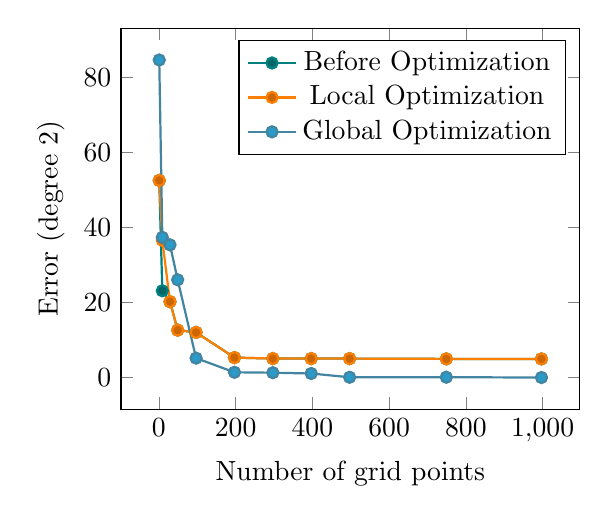
\begin{tikzpicture}
		\begin{axis}[
			xlabel = Number of grid points,
			ylabel = Error (degree 2),
			scale=0.85,
			cycle list name=exotic,
			legend pos=north east,
			]
			
			\addplot+[mark=*, style=thick] coordinates
			{(1,52.5) (9,23.124999999999993) (29,20.221948342338713) (49,12.642146873903034) (97,12.037968800252116) (197,5.324940782205941) (297,5.070573664357864) (397,5.059483529507994) (497,5.059483529509992) (749,4.981978981445401) (997,4.975134049661977) };
			
			\addplot+[mark=*, style=thick]  coordinates 
			{(1,52.5) (9,36.56247783900481) (29,20.221948342338713) (49,12.642146873903027) (97,12.037968800252123) (197,5.324940782205946) (297,5.070573664357985) (397,5.059483529510453) (497,5.059483529510453) (749,4.981978981455729) (997,4.975134049663653) };
			
			\addplot+[mark=*, style=thick]   coordinates 
			{(1,84.58773867867924) (9,37.34881542254573) (29,35.353118558881526) (49,26.048828056455157) (97,5.180279637187814) (197,1.4141172901666579) (297,1.3031251937216908) (397,1.0903873189756652) (497,0.08680369103412033) (749,0.10422400147368194) (997,0.020853342869873615) };
			
			\legend{Before Optimization, Local Optimization, Global Optimization}
			
		\end{axis}
	\end{tikzpicture}
	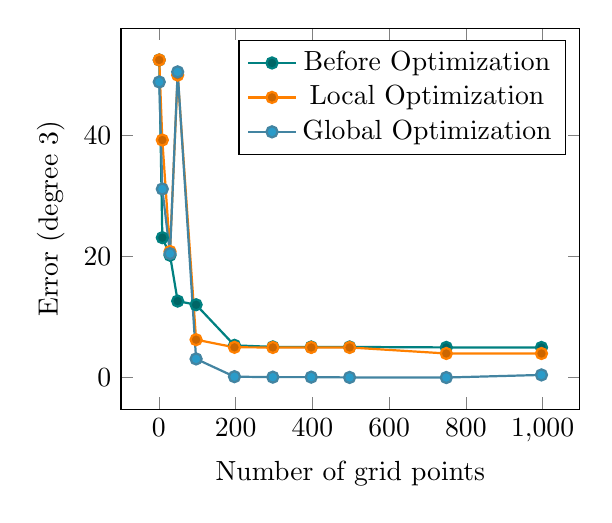
\begin{tikzpicture}
		\begin{axis}[
			xlabel = Number of grid points,
			ylabel = Error (degree 3),
			scale=0.85,
			cycle list name=exotic,
			legend pos=north east,
			]
			
			\addplot+[mark=*, style=thick] coordinates
			{(1,52.5) (9,23.124999999999986) (29,20.221948342338727) (49,12.642146873903025) (97,12.037968800252077) (197,5.324940782206068) (297,5.070573664356438) (397,5.059483529515382) (497,5.059483529505752) (749,4.9819789814573205) (997,4.975134049660271) };
			
			\addplot+[mark=*, style=thick]  coordinates 
			{(1,52.5) (9,39.26658373479667) (29,20.847171449176678) (49,49.99973745586844) (97,6.259687480962173) (197,5.002154846904871) (297,4.975751718068931) (397,4.975746034104377) (497,4.975697508130967) (749,3.980892241733912) (997,3.979835850885795) };
			
			\addplot+[mark=*, style=thick]   coordinates 
			{(1,48.864612088186476) (9,31.16918203994022) (29,20.48853217431511) (49,50.53387608332728) (97,3.0805866327728566) (197,0.14445847530268452) (297,0.06980177032781754) (397,0.06988725538127483) (497,0.02077395004058502) (749,0.003850124352695161) (997,0.4352002384999345) };
			
			\legend{Before Optimization, Local Optimization, Global Optimization}
			
		\end{axis}
	\end{tikzpicture}
	\centering
	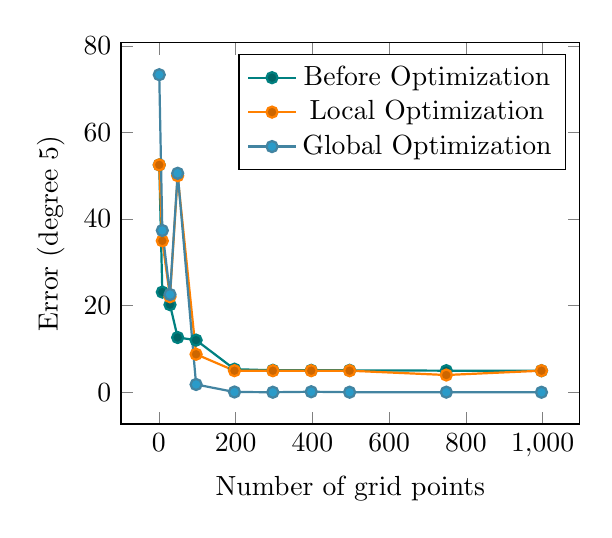
\begin{tikzpicture}
		\begin{axis}[
			xlabel = Number of grid points,
			ylabel = Error (degree 5),
			scale=0.85,
			cycle list name=exotic,
			legend pos=north east,
			]
			
			\addplot+[mark=*, style=thick] coordinates
			{(1,52.5) (9,23.124999999999996) (29,20.221948342338706) (49,12.642146873903044) (97,12.037968800252427) (197,5.324940782206359) (297,5.070573664363549) (397,5.059483529512068) (497,5.059483529510554) (749,4.981978981456664) (997,4.975134049668072) };
			
			\addplot+[mark=*, style=thick]  coordinates 
			{(1,52.5) (9,34.964270829168846) (29,22.048613242940117) (49,49.999815285630675) (97,8.771776029715767) (197,4.977579661397227) (297,4.9749420077761) (397,4.974930572100956) (497,4.974940210636003) (749,3.9798360656238323) (997,4.974790247773939) };
			
			\addplot+[mark=*, style=thick]   coordinates 
			{(1,73.32956404214876) (9,37.355007206361236) (29,22.57998988395788) (49,50.570154840256905) (97,1.7957114981045024) (197,0.059327067234512754) (297,0.0044097596433303465) (397,0.11308692978262513) (497,0.008066444905090009) (749,0.02197720207793452) (997,0.002142203898742423) };
			
			\legend{Before Optimization, Local Optimization, Global Optimization}
			
		\end{axis}
	\end{tikzpicture}
	\caption{ Optimization error for different algorithms depending on the number of grid points in two dimensions. The plots show the results with degree 2 (top left), degree 3 (top right) and degree 5 (bottom). The Rosenbrock function was used. }	
	\label{fig:Optimizer_results}
\end{figure}

In all three cases, the errors of the local and global optimizers first increase with increasing number of grid points until about 100 to 200 function evaluations are done. After that, both local and global optimization algorithms are at least as good as the result found by the sparse grid. With increasing number of grid points, the global optimization finds the best solution in all cases with degrees 2, 3, and 5.

One approach is to combine all three resulting points with their corresponding function value. The overall optimal point is then just set to the one with the smallest function value. \newline 

The input of the previous experiments were all just in two dimensions. The following ones analyze the impact of the dimension on the performance of the algorithm. Therefore, the Rastrigin function is optimized, again with increasing number of grid points. The degree of the B-splines used on the sparse grid is set to 5 and for the adaptivity parameter, we set $ \gamma = 0.85 $. The results are depicted in Figure \ref{fig:Dimensions_results}.


\begin{figure}[htbp!]
	\centering
	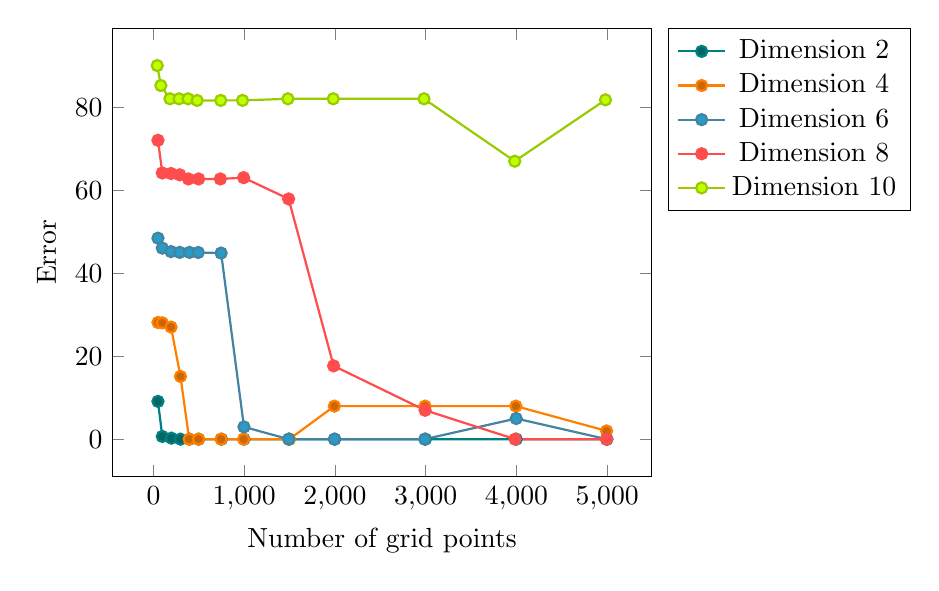
\begin{tikzpicture}
		\begin{axis}[
			xlabel = Number of grid points,
			ylabel = Error,
			scale=1,
			cycle list name=exotic,
			legend pos=outer north east,
			]
			
			\addplot+[mark=*, style=thick] coordinates
			{(49,9.101448500006125) (97,0.6579925771421742) (197,0.24877350577453328) (297,0.004037953576528253) (397,0.00025859422627760864) (497,1.7408297026122455e-13) (749,7.460698725481052e-14) (997,3.481659405224491e-13) (1497,5.044853423896711e-13) (1997,2.1316282072803006e-14) (2997,3.652389892749852e-06) (3997,2.8704901623655132e-05) (4997,5.787840197764794e-07) };
			
			\addplot+[mark=*, style=thick]  coordinates 
			{(49,28.11190602660223) (97,28.027731473104676) (193,27.012106473104676) (297,15.113252690760966) (393,9.600766347261924e-06) (497,1.6991705820146308e-09) (745,2.1316282072803006e-14) (993,8.952838470577262e-13) (1497,5.101696842757519e-12) (1993,7.959662418317201) (2993,7.959662532446124) (3993,7.959662444938445) (4993,1.989918226969806) };
			
			\addplot+[mark=*, style=thick]   coordinates 
			{(49,48.423119589928916) (97,46.02773147310465) (193,45.19017740517299) (289,45.000002956271466) (397,45.00000295627026) (493,44.97832419159962) (745,44.83586659446601) (997,2.9518635934690423) (1489,1.2755663192365319e-10) (1993,3.339550858072471e-13) (2989,3.609557097661309e-12) (3997,4.974795290848007) (4993,2.3494095557907713e-10) };
			
			\addplot+[mark=*, style=thick]  coordinates 
			{(49,72.00000000000047) (97,64.13062375846819) (193,63.995042024453646) (289,63.68474722559662) (385,62.68963603135439) (497,62.68978857181299) (737,62.688613023877224) (993,63.000000000740776) (1489,57.870967998853985) (1985,17.661726128773374) (2993,6.96530803395143) (3985,1.0274447959091049e-11) (4993,9.632833695150111e-07) };
			
			\addplot+[mark=*, style=thick]   coordinates 
			{(41,90.00000000000006) (81,85.19455718813529) (181,82.0037952623156) (281,81.99495932097409) (381,81.99495905766113) (481,81.59599881413277) (741,81.61443670251717) (981,81.61429574478895) (1481,81.99495913158995) (1981,81.99495935231735) (2981,81.99495919483614) (3981,66.96083466127668) (4981,81.74484728227361) };
			
			\legend{Dimension 2, Dimension 4, Dimension 6, Dimension 8, Dimension 10}
			
		\end{axis}
	\end{tikzpicture}
	\caption{ Error of the optimization depending on the number of grid points used for different dimensions of the Rastrigini function. }	
	\label{fig:Dimensions_results}
\end{figure}

The results show that with increasing dimensionality of the problem, more grid points are needed in order to reduce the error. The metric was again defined as the optimum found by the algorithm subtracted by the actual optimal value. \newline 

In conclusion, the adaptivity parameter, the degree of the B-splines on the sparse grid, and the dimensionality of the problem that is optimized, strongly influence the behavior of the sparse grid optimization. For the adaptivity parameter, a value with about $ \gamma = 0.85 $ is in general a good choice for a function that is not known in advance. With a higher degree, we can find the optimum a bit faster and for higher dimensionality, more refinement iterations of the sparse grid are needed. 


\section{Hyperparameter Optimization with Sparse Grids}

Now we replace the function, where we know the analytical optimum with the evaluation of a machine learning model. The biggest change is the much higher duration of one function call and the complexity of finding the analytical solution which is impossible due to the high number of network weights in neural networks. 

\subsection{Optimum Approximation with Sparse Grids}

The following plots show an example of a small neural network being evaluated on the diamonds dataset which is available on OpenML \cite{feurer-arxiv19a}. We used a model consisting of two fully connected layers, each made up of 30 neurons. In one batch, 100 data samples are processed. The two dimensional plot (see Figure \ref{fig:analysis_model_training}) depicts the network evaluation depending on the number of epochs used and the value for the learning rate of the Adam optimizer of the model. The loss of the network is calculated with the mean squared error. As pre-processing of the data, the numeric features of the input data is scaled with a standard scaler and the categorical features are one hot encoded. The target values are also scaled separately. For the evaluation metric, we chose the average result of 2-fold-cross validation with the mean absolute percentage error (MAPE). This metric is defined as 
\begin{equation}
 	\text{MAPE} = \frac{1}{n} \sum_{i=1}^{n}\left|\frac{y^i - y^i_{pred}}{y^i}\right|
\end{equation}
where $ y^i $ is the target value and $ y^i_{pred} $ is the predicted value of data point $ x^i $.

The interval of the epochs is $ [1, 40] $ and the learning rate is sampled equidistant and logarithmic between $ [10^{-10}, 10^{-1}] $. The resulting plot with the result depending on the epochs and the $ log_{10}(\text{learning rate}) $ can be seen in Figure \ref{fig:analysis_model_training}.

\begin{figure}[htbp!]
	\centering
	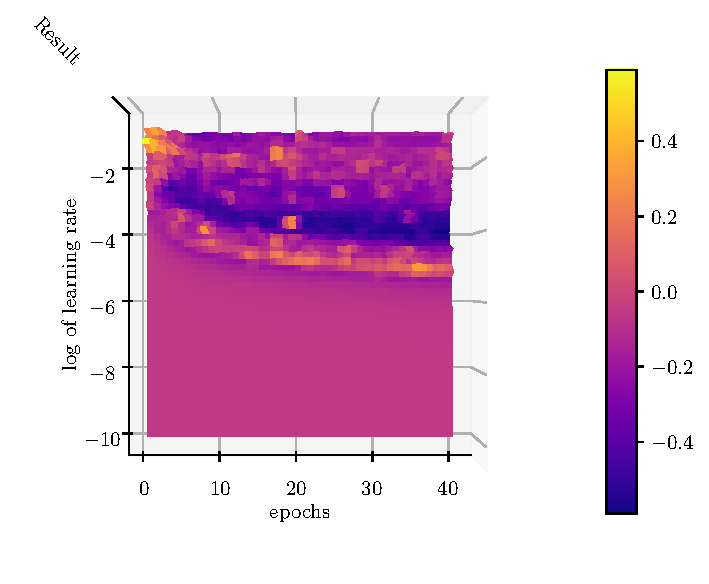
\includegraphics[width=0.48\textwidth]{figures/Results/Machine_learning/1000_evaluations/Network_above}
	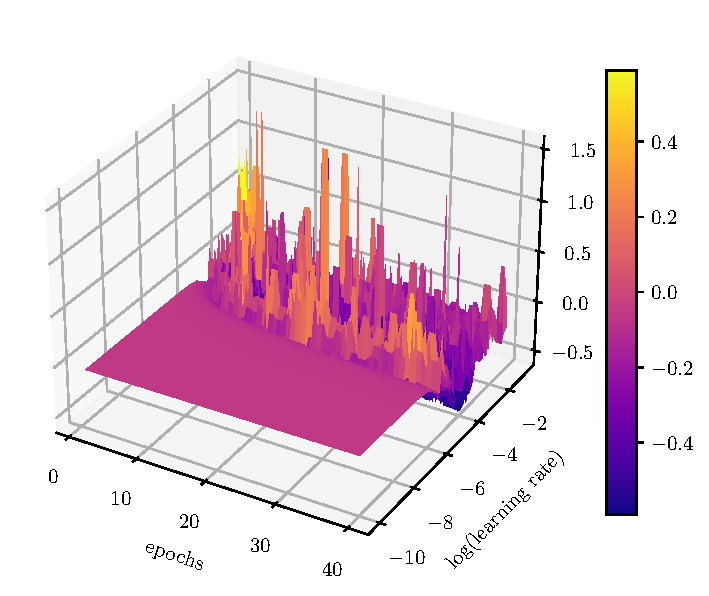
\includegraphics[width=0.48\textwidth]{figures/Results/Machine_learning/1000_evaluations/Network_normal}
	
	\caption{ 2-layer (with 30 neurons each) fully connected network evaluation on the diamonds dataset depending on the number of epochs and learning rate of the Adam optimizer. }
	\label{fig:analysis_model_training}
\end{figure}

In this plot, for each of epochs and learning rate, 100 different, equidistant values are sampled from the corresponding interval (linear sampling for epochs and log sampling for learning rate). All different combinations are evaluated leading to $ 100^2 = 10000 $ function evaluations. This took about 45 hours on a normal machine. Regarding the goal of hyperparameter optimization, this technique of trying all different combinations of distinct values is comparable to the grid search approach which is not very efficient. Although, the rough behavior of the machine learning model can be analyzed. The function is nearly constant for the learning rate between $ 10^{-6} $ and $ 10^{-10} $. This is caused by the Adam optimizer adjusting the weights of the network too slow in order to minimize the error. In the other half of the domain (learning rate between $ 10^{-1} $ and $ 10^{-5} $), a blue region where the smallest errors are achieved can be observed. This is where the combination between epochs and learning rate is very good for achieving good results. With this plot, a general observation can be made. However, it takes far too much time to analyze each problem with a plot like this. Additionally to the high effort, only the region of the minimum can be determined, not the optimal point itself. \newline

With this knowledge about the underlying function that has to be minimized, the behavior of the sparse grid can be analyzed. Figure \ref{fig:analysis_sparse_grid_with_machine_learning} depicts the generated grid colored corresponding to the function value for different adaptivity values and number of grid points. Note that the scale of the learning rate is the one interpreted by the sparse grid. The actual scale is logarithmic between $ 10^{-10} $ for $ 0.0 $ and $ 10 ^{-1} $ for $ 1.0 $. 

\begin{figure}[htbp!]
	\begin{subfigure}{\textwidth}
		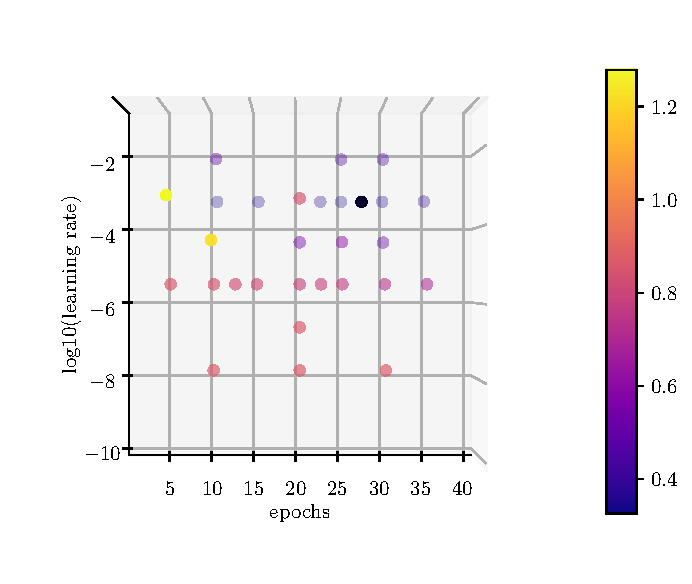
\includegraphics[width=0.48\textwidth]{figures/Results/Machine_learning/first_analysis/above_30_85}
		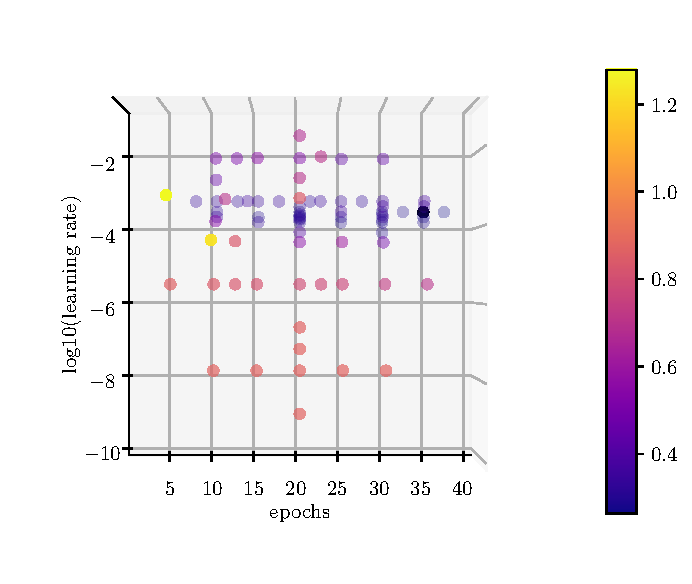
\includegraphics[width=0.48\textwidth]{figures/Results/Machine_learning/first_analysis/above_80_85}
		\caption{ Sparse grid generated with adaptivity parameter $ \gamma = 0.85 $ and number of grid points of 29 (left) and 77 (right). Most points are in the upper half for higher values of the learning rate. }
		\label{fig:analysis_sparse_grid_with_machine_learning_085}
	\end{subfigure}
	
	\begin{subfigure}{\textwidth}
		\includegraphics[width=0.48\textwidth]{figures/Results/Machine_learning/first_analysis/Above_30_5}
		\includegraphics[width=0.48\textwidth]{figures/Results/Machine_learning/first_analysis/Above_80_5}
		\caption{Sparse grid generated with adaptivity parameter $ \gamma = 0.5 $ and number of grid points of 29 (left) and 77 (right). Most points are in the upper right half for higher values of the learning rate and epochs between 25 and 30. }
		\label{fig:analysis_sparse_grid_with_machine_learning_05}
	\end{subfigure}

	\caption{ Analysis of sparse grid with machine learning evaluation for different adaptivity parameters ($ 0.85 $ \ref{fig:analysis_sparse_grid_with_machine_learning_085} and $ 0.5 $ \ref{fig:analysis_sparse_grid_with_machine_learning_05}), each with 29 and 77 grid points.}
	\label{fig:analysis_sparse_grid_with_machine_learning}
\end{figure}

In the first case with $ \gamma = 0.85 $, more grid points are generated in the upper half of the domain. A similar behavior can be observed for a higher number of grid points (\ref{fig:analysis_sparse_grid_with_machine_learning_085}, right). Especially in regions where the learning rate is about $ 0.0002 $ to $ 0.0003 $ (scale marked at $ 0.7 $), many grid points are refined. From the analysis in Figure \ref{fig:analysis_model_training}, there might be the optimal value. 

For a smaller adaptivity value of $ \gamma = 0.5 $, the sparse grid is much more adaptive as depicted in Figure \ref{fig:analysis_sparse_grid_with_machine_learning_05}. For both number of grid points $ 50 $ and $ 100 $, the most refined part of the sparse grid is at the same region. One important thing to observe here is that with higher adaptivity, a lower number of grid points is necessary to find one candidate of the optimum value. On the other hand, with lower adaptivity, more grid points are needed to find a good minimal value. 

However, as shown in Table \ref{tab:analysis_sparse_grid_with_machine_learning_results}, the best value is found with the configuration $ \gamma = 0.85 $ and number of grid points of 100. This means that lower adaptivity leads to better results.

\begin{table}[htbp!]
	\centering
	\begin{tabular}{| c c | c c | c |} 
		\hline
		$ \gamma $ & N &  Epochs & Learning rate & Result \\
		\hline
%		0.85 & 29 & 27 & 0.0005623413251903491 & 0.3259957134723667 \\
%		0.85 & 77 & 35 & 0.00029427271762092817 & \textbf{0.26339022070169354} \\
%		0.5 & 29 & 26 & 0.00015399265260594922 & 0.26837945729494134 \\
%		0.5 & 77 & 26 & 0.00015399265260594922 & 0.2683794572949415 \\
		0.85 & 29 & 27 & 0.00056 & 0.32599 \\
		0.85 & 77 & 35 & 0.00029 & \textbf{0.26339} \\
		0.5 & 29 & 26 & 0.00015 & 0.26837 \\
		0.5 & 77 & 26 & 0.00015 & 0.26837 \\
		\hline
	\end{tabular}
	\caption{ Best hyperparameter configuration found by the sparse grid with different adaptivity parameters and number of grid points. The best result is found with $ \gamma = 0.85 $ and 77 grid points. }
	\label{tab:analysis_sparse_grid_with_machine_learning_results}
\end{table}

The results shown in this table prove that too high adaptivity is not good for finding the smallest function value. However, when using higher adaptivity, the number of grid points has no big impact on finding the best solution in this case. This is because of the function shown in Figure \ref{fig:analysis_model_training}. In general, a higher adaptivity is good for finding a configuration faster. This can be useful in cases of hyperparameter optimization where not much time is available and a relatively good solution is enough. 

\subsection{Optimization on Sparse Grids}

By adding optimization methods like gradient descent or evolutionary algorithms, an even better approximation of the optimum might be found. In the following, the local and global optimization after the sparse grid generation is analyzed. 

One important thing to keep in mind is that given a certain budget $ N $ which can be the number of function evaluations, the algorithm may not take more than that to find the optimal point. With the additional optimization algorithm which takes $ c $ function evaluations, the number of grid points is then $ N - c $. 







